\documentclass{article}
\title{Atreus Keyboard Assembly: Lacquered Case}
\date{ }
\usepackage[right=2.5cm, left=2.5cm, top=1cm, bottom=1cm]{geometry}
\usepackage{graphicx}
\usepackage{parskip}
\pagenumbering{gobble}
\begin{document}
\maketitle
\vspace{-3em}

The wooden Atreus Keyboard case can be made with an oil/wax finish,
but if you have the patience to apply several coats of lacquer finish
you can get a very pleasing shiny look with a smoother texture.

\vspace{1em}
\noindent\makebox[\textwidth]{%
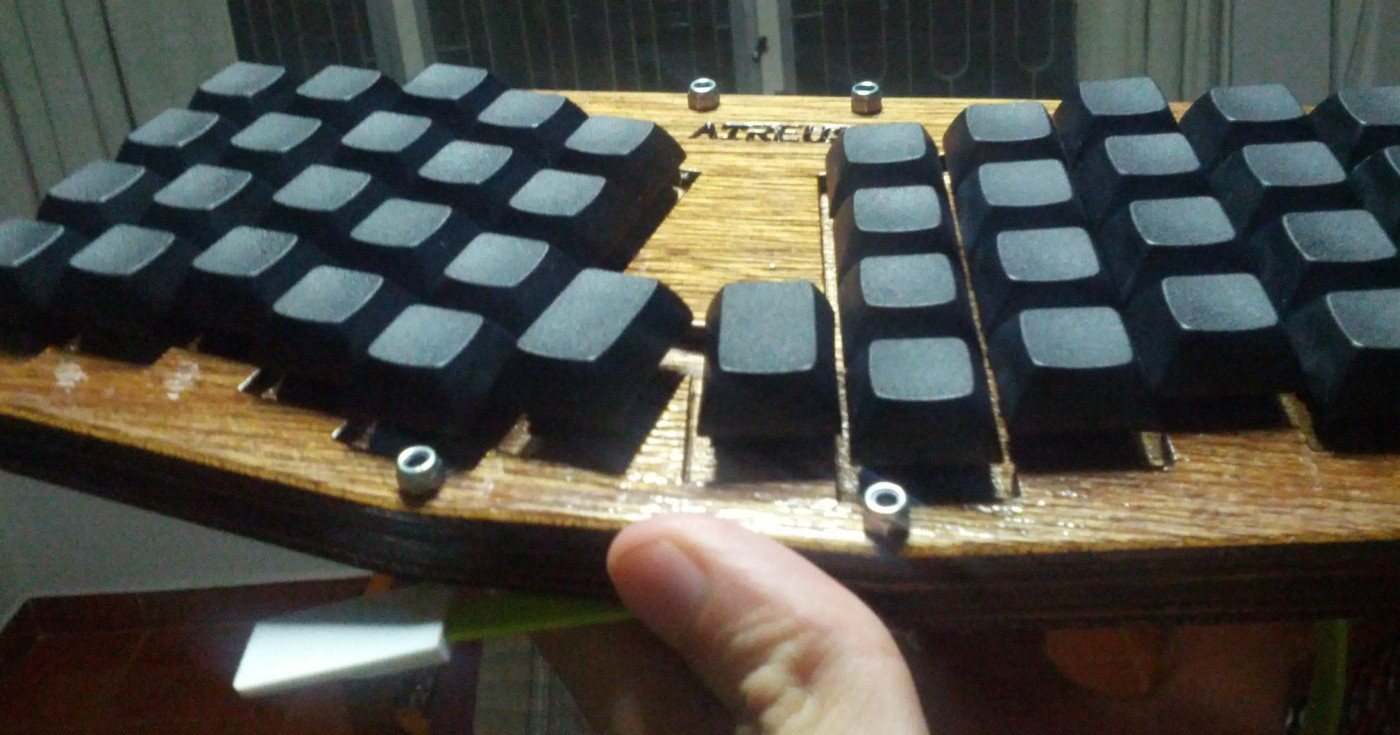
\includegraphics[width=0.7\linewidth]{lacquer.jpg}}
\vspace{1em}

You'll need a few items in addition to what's in the kit:

\begin{itemize}
\item Fine waterproof sandpaper (between 1000 and 2000 grit)
\item Can of spray lacquer (clear glossy recommended)
\item Newspaper or other material to spray on
\end{itemize}

Start by sanding everything with the 100-grit paper included in the
kit. Pay special attention to remove the scorch marks from the laser
cutting. Some people don't like the look of the exposed edges charred
from the laser cutter. You can choose to sand off the charring to
expose the layered ply or alternately cover it all with black ink from
a sharpie for a more consistent look if you prefer.

Once the case is sanded down all over with coarse sandpaper, find a
good place to spray the lacquer. It should be outdoors, or in a
well-ventilated garage if spraying outdoors is not feasible. Lay down
the newspaper with the pieces of the case on top of it. Spray your
first coat of lacquer to the face-up side of each piece. Try to use a
steady hand and keep the path of the spray overlapping itself just a
small amount as you go to and fro to minimize runs but still cover all
the area. The evenness of the spray matters less on the internal
surfaces of the case, so it's a good time to practice and get the hang
of it.

Check the lacquer directions to see how long your particular product
needs to dry; this can vary from half an hour to nearly a day. Once
your first coat is dry, flip each piece over and spray the other
side. Repeat for a second coat.

After the second coat, you can ignore all surfaces except for the top
of the top plate and the bottom of the bottom plate since only these
are exposed to the outside. At this point you can take in the switch
plate and continue the rest of the keyboard construction while you
wait for remaining coats to dry.

The outer surfaces should have between eight to ten coats applied total. As
you get to the later coats, the end result will be smoother if you can
keep them thinner. After your last coat dries, take your fine
sandpaper and soak it, then sand over the top and bottom surfaces
lightly. If you make any mistakes or are unhappy with the smoothness
of the finish, let it dry and add another layer of lacquer, then try
sanding it again.

As a final step after the case has dried from the wet sanding, take
the wax/oil mixture from the kit and spread some over the outer two
surfaces with your fingers, rubbing it into the finish as a
polish. Let the oil soak into the finish for a few hours. The end
result should look a bit like the wood of a guitar.

Congratulations; you should have a beautifully-finished case. Enjoy!

\end{document}
